% This document is code to produce the equations in the article:
% What is Your Estimand? Defining the Target Quantity Connects Statistical Evidence to Theory
% by Ian Lundberg, Rebecca Johnson, and Brandon Stewart
% Paper: https://doi.org/10.1177%2F00031224211004187
% Preprint: https://doi.org/10.31235/osf.io/ba67n
% Replication: https://doi.org/10.7910/DVN/ASGOVU

\documentclass[tikz]{standalone}
\newcommand\independent{\protect\mathpalette{\protect\independenT}{\perp}}
\def\independenT#1#2{\mathrel{\rlap{$#1#2$}\mkern2mu{#1#2}}}
\usepackage{color}
% === math packages ===
\usepackage[reqno]{amsmath}
\setcounter{tocdepth}{5}
\usepackage[pdftex]{hyperref}
\usepackage{amsthm}
\usepackage{framed}
\usepackage{amssymb,enumerate}
\usepackage[all]{xy}
%\usepackage{lscape}
\usepackage{tikz}
\usepackage{times}
\usetikzlibrary{fit,positioning,shapes,positioning,decorations.pathmorphing, decorations.pathreplacing}
\usetikzlibrary{arrows}
\newcommand{\indep}{{\bot\negthickspace\negthickspace\bot}}
\newcommand{\E}{{\rm I\kern-.3em E}}
\newcommand{\Var}{\text{Var}}
\newcommand{\V}{\text{V}}
\newcommand{\N}{\mathcal{N}}
\newcommand{\I}{\text{I}}
\newcommand{\Cov}{\text{Cov}}
\newcommand{\Cor}{\text{Cor}}
\renewcommand{\P}{\text{P}}
\newcommand{\mean}{\text{mean}}
\usepackage{color,setspace}
\newcommand\X{\mathbf{X}}

\begin{document}
    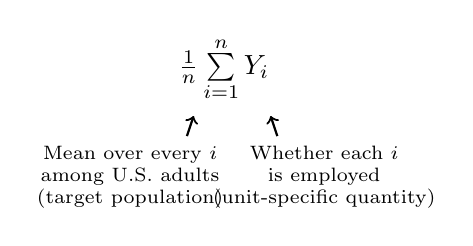
\begin{tikzpicture}[x = .85cm, y = .85cm]
    \node at (0,0) {$\frac{1}{n}\sum\limits_{i=1}^n Y_i$};
    \node[anchor = north, font = \scriptsize, align = center] at (-1.4,-1) {Mean over every $i$\\among U.S. adults\\(target population)};
    \node[anchor = north, font = \scriptsize, align = center] at (1.5,-1) {Whether each $i$\\is employed\\(unit-specific quantity)};
    \draw[->, thick] (-.55,-1) -- (-.45,-.7);
    \draw[->, thick] (.8,-1) -- (.7,-.7);
\end{tikzpicture}

    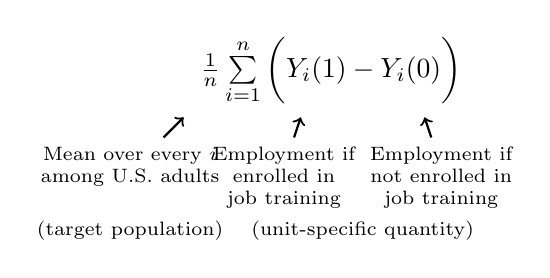
\begin{tikzpicture}[x = .85cm, y = .85cm]
    \node at (0,0) {$\frac{1}{n}\sum\limits_{i=1}^n \bigg(Y_i(1) - Y_i(0)\bigg)$};
    \node[anchor = north, font = \scriptsize, align = center] (mean) at (-3,-1) {Mean over every $i$\\among U.S. adults};
    \node[anchor = north, font = \scriptsize, align = center] at (-3,-2.1) {(target population)};
    \node[anchor = north, font = \scriptsize, align = center] at (-.7,-1) {Employment if\\enrolled in\\job training};
    \node[anchor = north, font = \scriptsize, align = center] at (1.65,-1) {Employment if\\not enrolled in\\job training};
    \node[anchor = north, font = \scriptsize, align = center] at (.475,-2.1) {(unit-specific quantity)};
    \draw[->, thick] (-2.5,-1) -- (-2.2,-.7);
    \draw[->, thick] (-.55,-1) -- (-.45,-.7);
    \draw[->, thick] (1.5,-1) -- (1.4,-.7);
\end{tikzpicture}

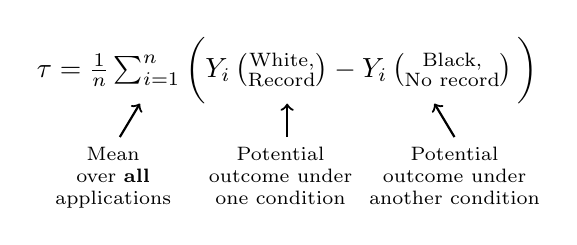
\begin{tikzpicture}[x = .85cm, y = .85cm]
    \node at (0,0) {$\tau = \frac{1}{n}\sum_{i=1}^n
    \bigg(
        Y_i\left(\substack{\text{White,}\\\text{Record}}\right) 
        - 
        Y_i\left(\substack{\text{Black,}\\\text{No record}}\right)
    \bigg)$};
    \node[anchor = north, font = \scriptsize, align = center] at (-2.6,-1) {Mean\\over \textbf{all}\\applications};
    \node[anchor = north, font = \scriptsize, align = center] at (-.1,-1) {Potential\\outcome under\\one condition};
    \node[anchor = north, font = \scriptsize, align = center] at (2.5,-1) {Potential\\outcome under\\another condition};
    \draw[->, thick] (-2.5,-1) -- (-2.2,-.5);
    \draw[->, thick] (0,-1) -- (0,-.5);
    \draw[->, thick] (2.5,-1) -- (2.2,-.5);
\end{tikzpicture}

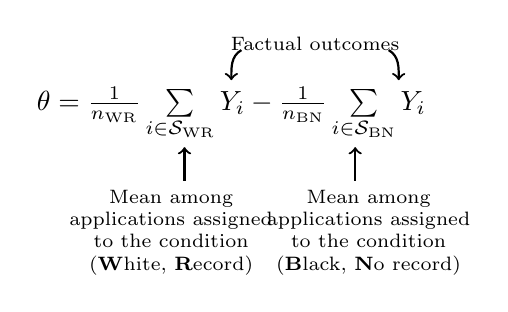
\begin{tikzpicture}[x = .85cm, y = .85cm]
    \node at (0,0) {$\theta = 
    \frac{1}{n_\text{WR}}\sum\limits_{i\in\mathcal{S}_\text{WR}}Y_i
        - 
    \frac{1}{n_\text{BN}}\sum\limits_{i\in\mathcal{S}_\text{BN}}Y_i
    $};
    \node[anchor = south, font = \scriptsize, align = center] at (1.25,.8) {Factual outcomes};
    %\draw[->, thick] (.4,1) -- (.2,.5);
    %\draw[->, thick] (2.2,1) -- (2.4,.5);
    \draw[->, thick] (.15,.95) to[out = 210, in = 90] (0,.5);
    \draw[->, thick] (2.35,.95) to[out = 330, in = 90] (2.5,.5);
    \node[anchor = north, font = \scriptsize, align = center] at (-.9,-1) {Mean among\\applications assigned\\to the condition\\(\textbf{W}hite, \textbf{R}ecord)};
    \draw[->, thick] (-.7,-1) -- (-.7,-.5);
    \node[anchor = north, font = \scriptsize, align = center] at (2.05,-1) {Mean among\\applications assigned\\to the condition\\(\textbf{B}lack, \textbf{N}o record)};
    \draw[->, thick] (1.85,-1) -- (1.85,-.5);
\end{tikzpicture}

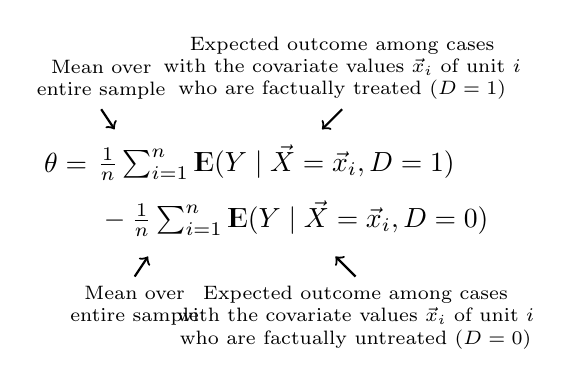
\begin{tikzpicture}[x = .85cm, y = .85cm]
\node[anchor = east] at (0.25,0) {$\theta = {}$};
\node[anchor = west] (first_mean) at (0,0) {$\frac{1}{n}\sum_{i=1}^n \E(Y\mid \vec{X} = \vec{x}_i, D = 1)$};
\node[anchor = north west] at (first_mean.south west) {${}- \frac{1}{n}\sum_{i=1}^n\E(Y\mid \vec{X} = \vec{x}_i, D = 0)$};
\node[anchor = south, align = center, font = \scriptsize] at (.2,.8) {Mean over\\entire sample};
\draw[->, thick] (.2, .8) -- (.4,.5);
\node[anchor = north, align = center, font = \scriptsize] at (.7,-1.7) {Mean over\\entire sample};
\draw[->, thick] (.7, -1.7) -- (.9,-1.4);
\node[anchor = south, align = center, font = \scriptsize] at (3.8,.8) {Expected outcome among cases\\with the covariate values $\vec{x}_i$ of unit $i$\\who are factually treated ($D = 1$)};
\draw[->, thick] (3.8, .8) -- (3.5,.5);
\node[anchor = north, align = center, font = \scriptsize] at (4,-1.7) {Expected outcome among cases\\with the covariate values $\vec{x}_i$ of unit $i$\\who are factually untreated ($D = 0$)};
\draw[->, thick] (4, -1.7) -- (3.7,-1.4);
\end{tikzpicture}

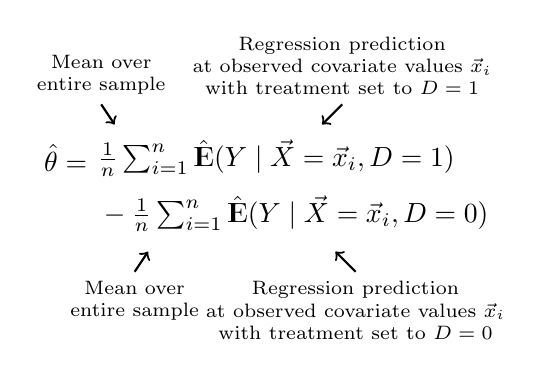
\begin{tikzpicture}[x = .85cm, y = .85cm]
\node[anchor = east] at (0.25,0) {$\hat\theta = {}$};
\node[anchor = west] (first_mean) at (0,0) {$\frac{1}{n}\sum_{i=1}^n \hat\E(Y\mid \vec{X} = \vec{x}_i, D = 1)$};
\node[anchor = north west] at (first_mean.south west) {${}- \frac{1}{n}\sum_{i=1}^n\hat\E(Y\mid \vec{X} = \vec{x}_i, D = 0)$};
\node[anchor = south, align = center, font = \scriptsize] at (.2,.8) {Mean over\\entire sample};
\draw[->, thick] (.2, .8) -- (.4,.5);
\node[anchor = north, align = center, font = \scriptsize] at (.7,-1.7) {Mean over\\entire sample};
\draw[->, thick] (.7, -1.7) -- (.9,-1.4);
\node[anchor = south, align = center, font = \scriptsize] at (3.8,.8) {Regression prediction\\at observed covariate values $\vec{x}_i$\\with treatment set to $D = 1$};
\draw[->, thick] (3.8, .8) -- (3.5,.5);
\node[anchor = north, align = center, font = \scriptsize] at (4,-1.7) {Regression prediction\\at observed covariate values $\vec{x}_i$\\with treatment set to $D = 0$};
\draw[->, thick] (4, -1.7) -- (3.7,-1.4);
\end{tikzpicture}

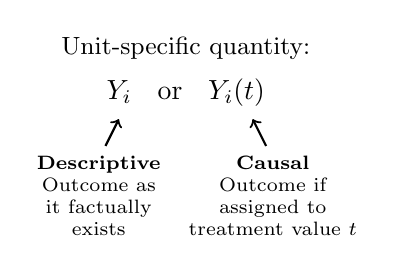
\begin{tikzpicture}[x = .85cm, y = .85cm]
\node[align = center] (y) at (0,0) {$Y_i\hspace{6pt}$ or $\hspace{6pt}Y_i(t)$};
\node[align = center, anchor = south, font = \small] at (y.north) {Unit-specific quantity:};
\node[anchor = north, font = \scriptsize, align = center] at (-1.3,-.8) {\textbf{Descriptive}\\Outcome as\\it factually\\exists};
\draw[->, thick] (-1.2,-.8) -- (-1,-.4);
\node[anchor = north, font = \scriptsize, align = center] at (1.3,-.8) {\textbf{Causal}\\Outcome if\\assigned to\\treatment value $t$};
\draw[->, thick] (1.2,-.8) -- (1,-.4);
\end{tikzpicture}

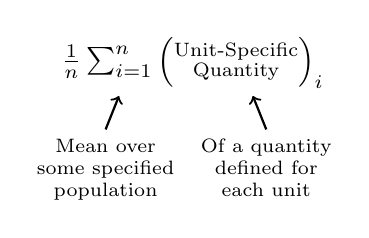
\begin{tikzpicture}[x = .85cm, y = .85cm]
\node at (0,0) {$\frac{1}{n}\sum_{i=1}^n \left(\substack{\text{Unit-Specific}\\\text{Quantity}}\right)_i$};
\node[anchor = north, align = center, font = \scriptsize] at (-1.3,-1) {Mean over\\some specified\\population};
\node[anchor = north, align = center, font = \scriptsize] at (1.1,-1) {Of a quantity\\defined for\\each unit};
\draw[->, thick] (-1.3,-1) -- (-1.1,-.5);
\draw[->, thick] (1.1,-1) -- (.9,-.5);
\end{tikzpicture}

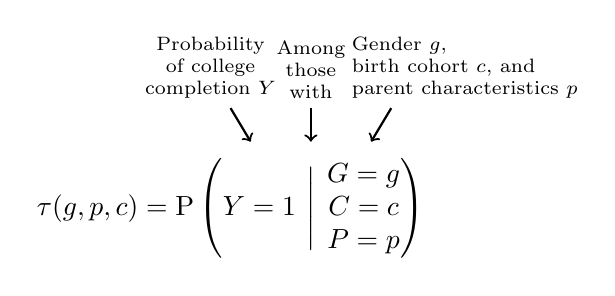
\begin{tikzpicture}[x = .85cm, y = .85cm]
\node at (0,0) {$\tau(g,p,c) = \P\left(Y = 1 \hspace{4pt}\Bigg\vert\hspace{4pt} \begin{matrix}G = g\\C = c\\P = p\end{matrix}\right)$};
\node[anchor = south, align = center, font = \scriptsize] at (-.3,1.5) {Probability\\of college\\completion $Y$};
\draw[->, thick] (0,1.5) -- (.3,1);
\node[anchor = south, align = center, font = \scriptsize] at (1.2,1.5) {Among\\those\\with};
\draw[->, thick] (1.2,1.5) -- (1.2,1);
\node[anchor = south, align = left, font = \scriptsize] at (3.5,1.5) {Gender $g$,\\birth cohort $c$, and\\parent characteristics $p$};
\draw[->, thick] (2.4,1.5) -- (2.1,1);
\end{tikzpicture}

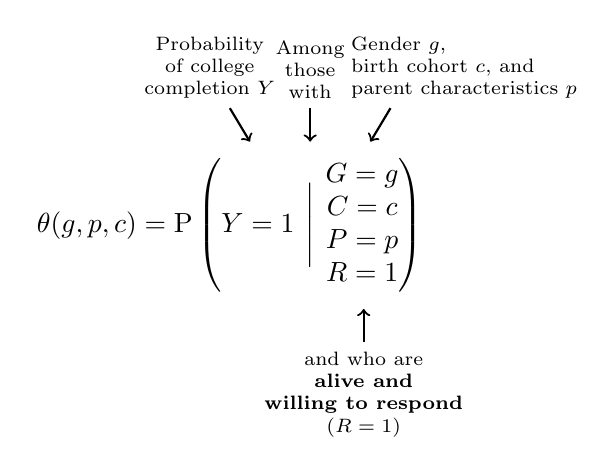
\begin{tikzpicture}[x = .85cm, y = .85cm]
\node at (0,-.25) {$\theta(g,p,c) = \P\left(Y = 1 \hspace{4pt}\Bigg\vert\hspace{4pt} \begin{matrix}G = g\\C = c\\P = p\\R = 1\end{matrix}\right)$};
\node[anchor = south, align = center, font = \scriptsize] at (-.3,1.5) {Probability\\of college\\completion $Y$};
\draw[->, thick] (0,1.5) -- (.3,1);
\node[anchor = south, align = center, font = \scriptsize] at (1.2,1.5) {Among\\those\\with};
\draw[->, thick] (1.2,1.5) -- (1.2,1);
\node[anchor = south, align = left, font = \scriptsize] at (3.5,1.5) {Gender $g$,\\birth cohort $c$, and\\parent characteristics $p$};
\draw[->, thick] (2.4,1.5) -- (2.1,1);
\node[anchor = north, align = center, font = \scriptsize] at (2,-2) {and who are\\\textbf{alive and}\\\textbf{willing to respond}\\($R = 1$)};
\draw[->, thick] (2,-2) -- (2,-1.5);
\end{tikzpicture}

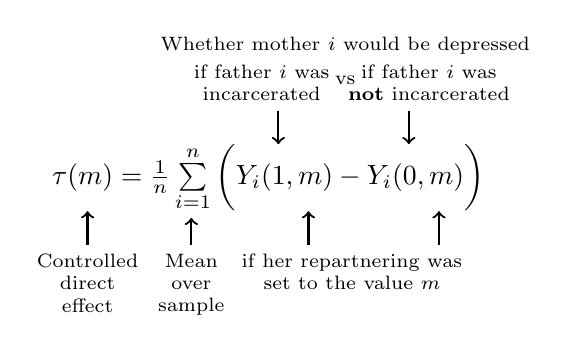
\begin{tikzpicture}[x = .85cm, y = .85cm]
\node at (0,0) {$\tau(m) = \frac{1}{n}\sum\limits_{i=1}^n\bigg(Y_i(1,m) - Y_i(0,m)\bigg)$};
\node[anchor = north, font = \scriptsize, align = center] at (-2.7,-1) {Controlled\\direct\\effect};
\draw[->, thick] (-2.7,-1) -- (-2.7,-.5);
\node[anchor = north, font = \scriptsize, align = center] at (-1.15,-1) {Mean\\over\\sample};
\draw[->, thick] (-1.15,-1) -- (-1.15,-.6);
\node[anchor = south, font = \scriptsize, align = center] at (1.15,1.7) {Whether mother $i$ would be depressed};
\node[anchor = south, font = \scriptsize, align = center] at (-.1,1) {if father $i$ was\\incarcerated};
\node[anchor = south, font = \scriptsize, align = center] at (1.15,1.25) {vs};
\node[anchor = south, font = \scriptsize, align = center] at (2.4,1) {if father $i$ was\\\textbf{not} incarcerated};
\draw[->, thick] (.15,1) -- (.15,.5);
\draw[->, thick] (2.1,1) -- (2.1,.5);
\node[anchor = north, font = \scriptsize, align = center] at (1.25,-1) {if her repartnering was\\set to the value $m$};
\draw[->, thick] (.6,-1) -- (.6,-.5);
\draw[->, thick] (2.55,-1) -- (2.55,-.5);
\end{tikzpicture}

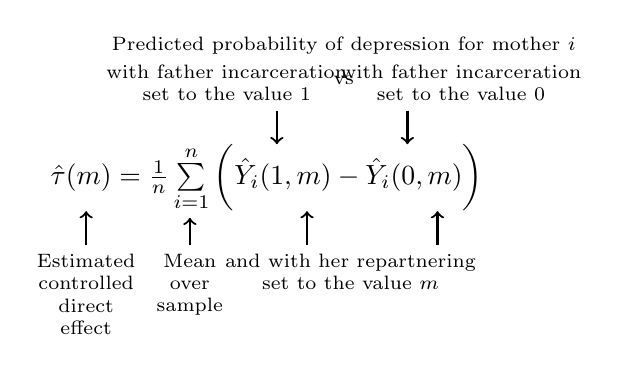
\begin{tikzpicture}[x = .85cm, y = .85cm]
\node at (0,0) {$\hat\tau(m) = \frac{1}{n}\sum\limits_{i=1}^n\bigg(\hat{Y}_i(1,m) - \hat{Y}_i(0,m)\bigg)$};
\node[anchor = north, font = \scriptsize, align = center] at (-2.7,-1) {Estimated\\controlled\\direct\\effect};
\draw[->, thick] (-2.7,-1) -- (-2.7,-.5);
\node[anchor = north, font = \scriptsize, align = center] at (-1.15,-1) {Mean\\over\\sample};
\draw[->, thick] (-1.15,-1) -- (-1.15,-.6);
\node[anchor = south, font = \scriptsize, align = center] at (1.15,1.7) {Predicted probability of depression for mother $i$};
\node[anchor = south, font = \scriptsize, align = center] at (-.6,1) {with father incarceration\\set to the value 1};
\node[anchor = south, font = \scriptsize, align = center] at (1.15,1.25) {vs};
\node[anchor = south, font = \scriptsize, align = center] at (2.9,1) {with father incarceration\\set to the value 0};
\draw[->, thick] (.15,1) -- (.15,.5);
\draw[->, thick] (2.1,1) -- (2.1,.5);
\node[anchor = north, font = \scriptsize, align = center] at (1.25,-1) {and with her repartnering\\set to the value $m$};
\draw[->, thick] (.6,-1) -- (.6,-.5);
\draw[->, thick] (2.55,-1) -- (2.55,-.5);
\end{tikzpicture}

\end{document}